Chương này trình bày các khái niệm nền tảng về Federated Learning và đi sâu phân tích cơ sở toán học của các thuật toán tổng hợp trọng số. Phần đầu sẽ giới thiệu thuật toán kinh điển FedAvg, đóng vai trò là mốc cơ sở (baseline). Phần tiếp theo sẽ phân tích thuật toán tiên tiến FedLWS, một phương pháp mới được đề xuất năm 2025 giúp cải thiện khả năng tổng quát hóa thông qua cơ chế co trọng số thích ứng.

\section{Tổng quan về Federated Learning}
Học máy liên kết (\ac{fl}) là một mô hình huấn luyện máy học phi tập trung, cho phép nhiều thiết bị (clients) cộng tác để học một mô hình chia sẻ toàn cầu mà vẫn giữ dữ liệu huấn luyện nằm cục bộ trên thiết bị \cite{McMahan2017}. Mục tiêu của \ac{fl} là tối ưu hóa hàm mục tiêu có dạng tổng hữu hạn:
\begin{equation}
    \min_{w \in \mathbb{R}^d} f(w) \quad \text{với} \quad f(w) \stackrel{\text{def}}{=} \frac{1}{n} \sum_{i=1}^{n} f_i(w)
\end{equation}
Trong đó, $f_i(w) = \ell(x_i, y_i; w)$ là hàm mất mát (loss function) trên mẫu dữ liệu $(x_i, y_i)$ với tham số mô hình $w$ \cite{McMahan2017}.


\section{Thuật toán Federated Averaging (FedAvg)}
\label{sec:FedAvg}

\subsection{Tổng quan và Cơ sở lý thuyết}
\textbf{Federated Averaging (FedAvg)}, được đề xuất bởi McMahan và cộng sự vào năm 2017, là thuật toán tối ưu hóa nền tảng cho Học máy liên kết (\ac{fl}) \cite{McMahan2017}. Thuật toán này ra đời nhằm giải quyết bài toán tối ưu hóa hàm mục tiêu toàn cầu $f(w)$ mà không cần truy cập trực tiếp vào dữ liệu thô nằm phân tán trên các thiết bị.

Về mặt toán học, mục tiêu của FedAvg là tìm tham số $w \in \mathbb{R}^d$ để tối thiểu hóa hàm mất mát tổng hợp:
\begin{equation}
    \min_{w} f(w) \quad \text{với} \quad f(w) \stackrel{\text{def}}{=} \sum_{k=1}^{K} \frac{n_k}{n} F_k(w)
\end{equation}
Trong đó:
\begin{itemize}
    \item $K$ là tổng số lượng client tham gia.
    \item $n_k$ là số lượng mẫu dữ liệu tại client $k$, và $n = \sum_{k} n_k$ là tổng dữ liệu toàn hệ thống.
    \item $F_k(w) = \frac{1}{n_k} \sum_{i \in \mathcal{P}_k} \ell(x_i, y_i; w)$ là hàm mất mát cục bộ (Local Loss Function) trên tập dữ liệu $\mathcal{P}_k$ của client $k$.
\end{itemize}

Động lực chính của FedAvg là khắc phục hạn chế về chi phí truyền thông của phương pháp tiền nhiệm \textit{FederatedSGD}. Thay vì đồng bộ hóa gradient sau mỗi bước tính toán đơn lẻ, FedAvg cho phép client thực hiện nhiều vòng lặp huấn luyện (epochs) để tính toán một cập nhật trọng số "chất lượng hơn" trước khi gửi đi, qua đó giảm thiểu số lần giao tiếp với máy chủ \cite{McMahan2017}.

\subsection{Quy trình hoạt động chi tiết}
Quá trình huấn luyện của FedAvg là một quy trình lặp (iterative process) gồm $T$ vòng giao tiếp (communication rounds). Tại mỗi vòng $t$, các bước thực hiện cụ thể như sau:

{Bước 1: Lựa chọn và Phân phối (Selection \& Broadcast)}
Tại đầu vòng $t$, máy chủ trung tâm (Server) chọn ngẫu nhiên một tập hợp con $S_t$ gồm $m$ client từ tổng số $K$ client khả dụng, với tỷ lệ tham gia $C$ ($m = \max(C \cdot K, 1)$). 
Máy chủ gửi tham số mô hình toàn cầu hiện tại $w_t$ đến tất cả các clients trong tập $S_t$.

{Bước 2: Tối ưu hóa cục bộ (Local Client Update)}
Mỗi client $k \in S_t$ nhận tham số $w_t$ và sao chép thành tham số cục bộ: $w_{t}^k \leftarrow w_t$.
Client thực hiện huấn luyện mô hình trên dữ liệu riêng $\mathcal{P}_k$ bằng thuật toán \textit{Stochastic Gradient Descent (SGD)}. Quá trình này diễn ra trong $E$ epochs (kỷ nguyên) với kích thước batch $B$ và tốc độ học $\eta$.

Quy tắc cập nhật cho mỗi bước lặp cục bộ (với batch dữ liệu $b \subset \mathcal{P}_k$):
\begin{equation}
    w^k \leftarrow w^k - \eta \nabla F_k(w^k; b)
\end{equation}
Sau khi hoàn thành $E$ epochs, client thu được bộ tham số đã cập nhật $w_{t+1}^k$.

\textit{Lưu ý:} Nếu $E=1$ và $B=n_k$ (full-batch), thuật toán trở về tương đương với FedSGD. Việc tăng $E > 1$ chính là chìa khóa giúp FedAvg hội tụ nhanh hơn về mặt truyền thông \cite{McMahan2017}.

{Bước 3: Tải lên tham số (Upload)}
Các client gửi vector tham số $w_{t+1}^k$ (hoặc vector chênh lệch $\Delta w^k = w_{t+1}^k - w_t$) trở lại máy chủ. Chỉ có trọng số mô hình được truyền đi, đảm bảo tính riêng tư dữ liệu.

{Bước 4: Tổng hợp trọng số (Aggregation)}
Máy chủ cập nhật mô hình toàn cầu bằng cách tính trung bình có trọng số (Weighted Averaging) các tham số nhận được. Trọng số quy định mức độ đóng góp của client dựa trên lượng dữ liệu sở hữu:
\begin{equation}
    w_{t+1} \leftarrow \sum_{k \in S_t} \frac{n_k}{n_{S_t}} w_{t+1}^k
\end{equation}
Trong đó $n_{S_t} = \sum_{k \in S_t} n_k$. Tham số $w_{t+1}$ được dùng làm đầu vào cho vòng $t+1$.

\begin{center}
    \begin{minipage}{\linewidth} % Dùng minipage để bó ảnh và caption lại với nhau
        \centering
        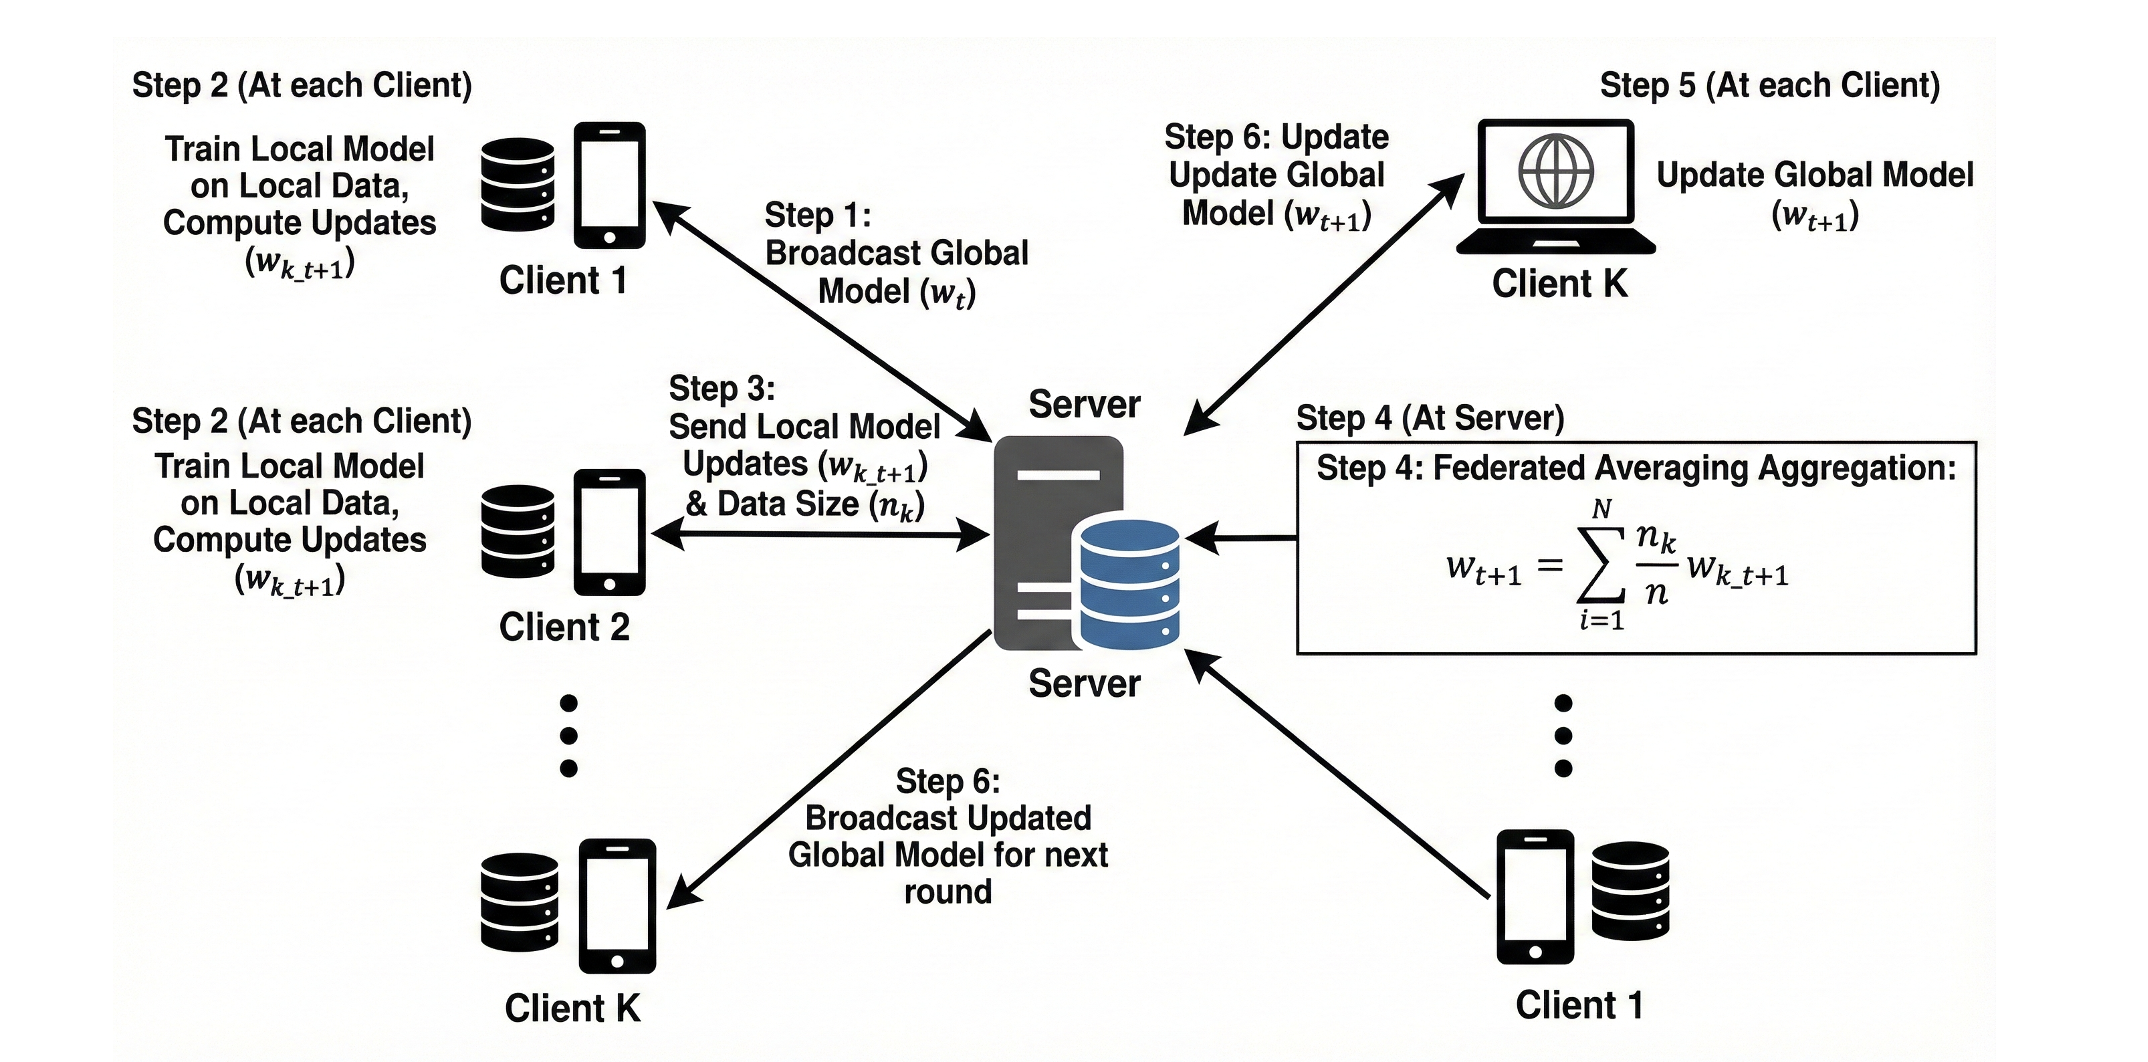
\includegraphics[width=0.7\textwidth]{img/fedavg_workflow.png}
        \captionof{figure}{Sơ đồ quy trình 4 bước của FedAvg: (1) Server phân phối, (2) Client cập nhật cục bộ, (3) Upload tham số, (4) Server tổng hợp \cite{McMahan2017}.}
        \label{fig:fedavg_workflow}
    \end{minipage}
\end{center}

\subsection{Phân tích Ưu và Nhược điểm}
\begin{itemize}
    \item \textbf{Ưu điểm:}
    \begin{itemize}
        \item \textbf{Hiệu quả truyền thông:} FedAvg giảm đáng kể tần suất giao tiếp so với SGD phân tán truyền thống. Thực nghiệm cho thấy FedAvg có thể giảm từ 10-100 lần số vòng lặp cần thiết để đạt độ chính xác tương đương trên các mô hình CNN \cite{McMahan2017}.
        \item \textbf{Tính riêng tư:} Dữ liệu thô được giữ lại hoàn toàn tại biên (edge devices).
        \item \textbf{Khả năng mở rộng:} Cơ chế chọn mẫu ngẫu nhiên (client sampling) cho phép hệ thống hoạt động tốt ngay cả khi số lượng thiết bị lên tới hàng triệu.
    \end{itemize}
    
    \item \textbf{Nhược điểm:}
    \begin{itemize}
        \item \textbf{Vấn đề Client Drift (Trôi dạt mô hình):} Đây là hạn chế lớn nhất. Trong môi trường dữ liệu Non-IID (phân phối dữ liệu khác nhau giữa các client), hàm tối ưu cục bộ $F_k(w)$ sẽ khác xa hàm tối ưu toàn cầu $f(w)$. Khi thực hiện nhiều bước cập nhật cục bộ ($E$ lớn), $w^k$ sẽ hội tụ về cực tiểu riêng của client đó thay vì cực tiểu chung, dẫn đến mô hình toàn cầu bị phân kỳ hoặc giảm độ chính xác \cite{McMahan2017}.
        \item \textbf{Tắc nghẽn do thiết bị chậm (Stragglers):} Quá trình tổng hợp phải chờ đợi client chậm nhất trong tập $S_t$ hoàn thành, gây lãng phí tài nguyên của các thiết bị nhanh hơn.
    \end{itemize}
\end{itemize}

\section{Thuật toán FedLWS (Federated Layer-wise Weight Shrinking)}
\label{sec:FedLWS}

\subsection{Tổng quan và Động lực nghiên cứu}
\textbf{Federated Learning with Layer-wise Weight Shrinking (FedLWS)}, được đề xuất bởi Shi và các cộng sự tại hội nghị ICLR 2025, là một phương pháp tối ưu hóa tiên tiến nhằm giải quyết vấn đề \textit{Client Drift} trong môi trường dữ liệu Non-IID \cite{Shi2025LWS}.

Động lực của FedLWS xuất phát từ một quan sát thực nghiệm sâu sắc về kiến trúc mạng nơ-ron sâu (Deep Neural Networks): "Độ nhạy cảm của các lớp mạng đối với sự không đồng nhất dữ liệu là không giống nhau".
\begin{itemize}
    \item Các lớp nông (Shallow layers - gần đầu vào): Thường học các đặc trưng cấp thấp (cạnh, góc, vân bề mặt) mang tính phổ quát, ít bị thay đổi giữa các client.
    \item Các lớp sâu (Deep layers - gần đầu ra): Chịu trách nhiệm phân loại dựa trên ngữ nghĩa cao cấp, do đó rất nhạy cảm và dễ bị lệch hướng (drift) khi dữ liệu cục bộ mất cân bằng nhãn (label distribution skew).
\end{itemize}

FedAvg thất bại trong việc nắm bắt sự tinh tế này vì nó áp dụng cơ chế trung bình cào bằng cho tất cả các lớp. FedLWS khắc phục điều này bằng cách áp dụng cơ chế "co trọng số" (weight shrinking) với tỷ lệ khác nhau cho từng lớp dựa trên độ ổn định của chúng.

\subsection{Cơ sở Toán học và Quy trình thực hiện}
Giả sử mô hình toàn cầu $w$ được cấu thành từ $L$ lớp mạng, ký hiệu là $\{w^1, w^2, ..., w^L\}$. Tại vòng giao tiếp $t$, sau khi các client thực hiện huấn luyện cục bộ và gửi cập nhật $\Delta w_k^t = w_k^{t+1} - w^t$ về máy chủ, FedLWS thực hiện quy trình tổng hợp 3 bước như sau:

{Bước 1: Tính toán Phương sai theo lớp (Layer-wise Variance)}
Máy chủ đo lường mức độ "bất đồng" giữa các client tại từng lớp mạng $l$ bằng cách tính phương sai của các vector cập nhật. Nếu các client cập nhật lớp $l$ theo các hướng quá khác nhau, phương sai sẽ cao, báo hiệu sự mất ổn định do dữ liệu Non-IID.
Công thức tính phương sai lớp $l$:
\begin{equation}
    \sigma_l^t = \frac{1}{K} \sum_{k=1}^{K} \left\| \Delta w_k^{l, t} - \overline{\Delta w^{l, t}} \right\|_2^2
\end{equation}
Trong đó $\overline{\Delta w^{l, t}}$ là trung bình cập nhật của lớp $l$.

{Bước 2: Xác định Hệ số Co (Shrinking Factor)}
Dựa trên phương sai $\sigma_l^t$, thuật toán tính toán một hệ số co $\alpha_l^t \in (0, 1]$ cho từng lớp. Nguyên tắc là: "Lớp nào biến động mạnh (phương sai lớn) thì co nhiều, lớp nào ổn định thì giữ nguyên".
Hàm tính hệ số co được đề xuất như sau:
\begin{equation}
    \alpha_l^t = \frac{1}{1 + \beta \cdot \exp(\gamma \cdot \sigma_l^t)}
\end{equation}
Trong đó $\beta$ và $\gamma$ là các siêu tham số kiểm soát độ nhạy của hàm co. Khi $\sigma_l^t \to 0$ (ổn định), $\alpha_l^t \to 1$ (giữ nguyên). Khi $\sigma_l^t$ lớn (bất ổn), $\alpha_l^t \to 0$ (giảm bớt sự đóng góp).

{Bước 3: Tổng hợp Thích ứng (Adaptive Aggregation)}
Máy chủ cập nhật mô hình toàn cầu bằng cách áp dụng hệ số co vào công thức trung bình trọng số. Thay vì cộng trực tiếp, các cập nhật sẽ được "làm mềm" (dampened) để tránh việc mô hình toàn cầu bị kéo lệch quá xa bởi các client cực đoan:
\begin{equation}
    w^{l, t+1} = w^{l, t} + \alpha_l^t \cdot \sum_{k=1}^{K} \frac{n_k}{n} \Delta w_k^{l, t}
\end{equation}

\begin{center}
    \begin{minipage}{\linewidth}
        \centering
        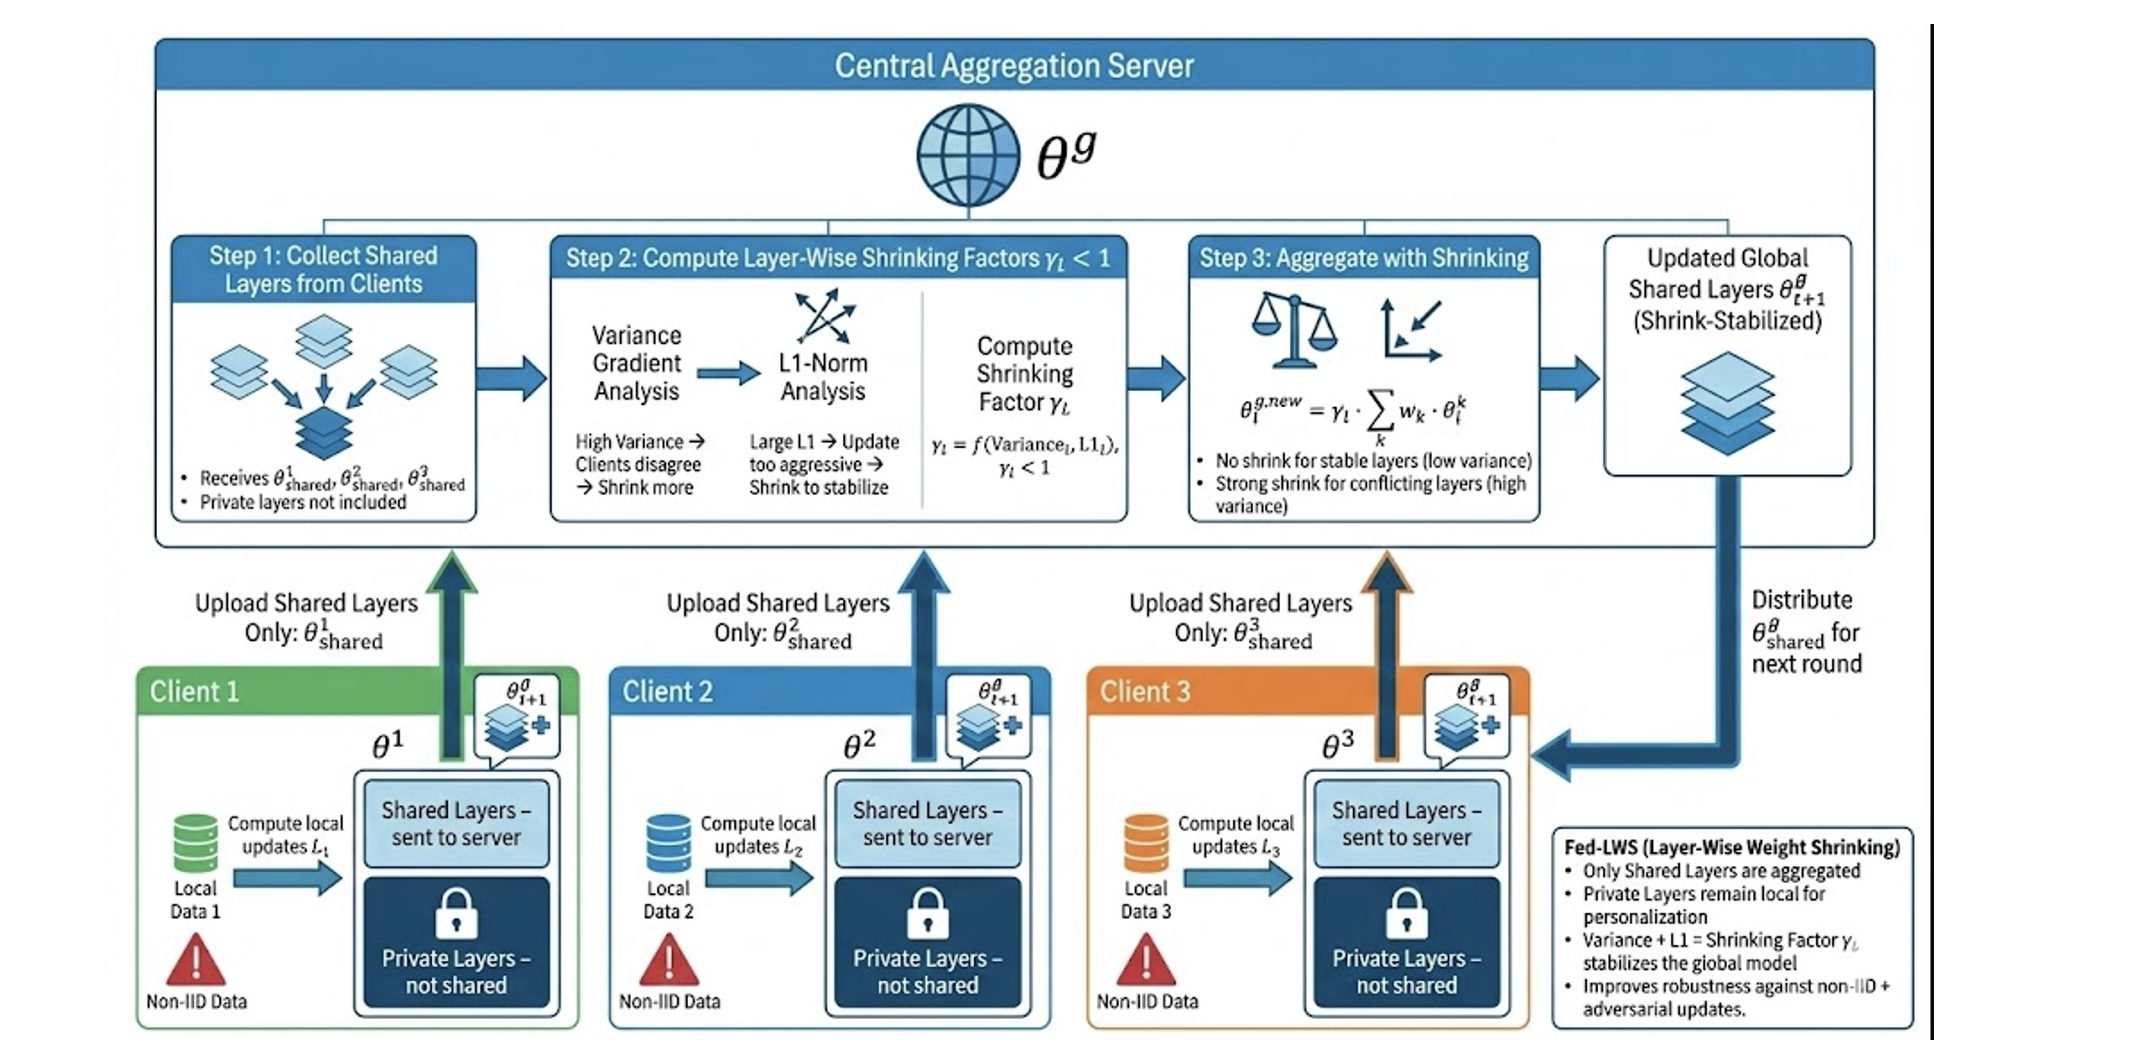
\includegraphics[width=0.85\textwidth]{img/fedlws_mechanism.png}
        \captionof{figure}{Cơ chế hoạt động của FedLWS: Các lớp sâu (gần output) có phương sai cập nhật lớn (màu đỏ) sẽ bị áp dụng hệ số co mạnh hơn để ổn định mô hình toàn cầu \cite{Shi2025LWS}.}
        \label{fig:fedlws_mechanism}
    \end{minipage}
\end{center}

\subsection{Phân tích Ưu và Nhược điểm}
\begin{itemize}
    \item \textbf{Ưu điểm:}
    \begin{itemize}
        \item \textbf{Cải thiện độ chính xác trên Non-IID:} Bằng cách kìm hãm các lớp nhạy cảm (thường là nguyên nhân chính gây Client Drift), FedLWS giúp mô hình hội tụ ổn định hơn và đạt độ chính xác cao hơn so với FedAvg (thực nghiệm cho thấy tăng ~2-3% trên CIFAR-10) \cite{Shi2025LWS}.
        \item \textbf{Không cần dữ liệu Proxy:} Khác với một số phương pháp yêu cầu server phải có một tập dữ liệu nhỏ để tinh chỉnh (như FedDF), FedLWS hoàn toàn dựa trên thống kê của trọng số mô hình, đảm bảo tính thực tế khi triển khai.
        \item \textbf{Chi phí truyền thông không đổi:} Không yêu cầu client gửi thêm bất kỳ thông tin phụ trợ nào ngoài tham số mô hình.
    \end{itemize}
    
    \item \textbf{Nhược điểm:}
    \begin{itemize}
        \item \textbf{Chi phí tính toán tại Server:} Máy chủ phải thực hiện tính toán phương sai và hệ số co cho từng lớp tại mỗi vòng lặp. Tuy nhiên, chi phí này là không đáng kể so với chi phí huấn luyện.
        \item \textbf{Thêm siêu tham số:} Việc lựa chọn $\beta, \gamma$ phù hợp có thể yêu cầu quá trình tinh chỉnh (tuning) dựa trên từng bộ dữ liệu cụ thể.
    \end{itemize}
\end{itemize}



\section{Thuật toán FedAWA (Federated Learning with Adaptive Weight Aggregation)}
\label{sec:FedAWA}

\subsection{Tổng quan và Động lực nghiên cứu}
\textbf{FedAWA (Federated Learning with Adaptive Weight Aggregation)}, được đề xuất bởi Shi và các cộng sự (2025), là một phương pháp tiếp cận mới nhằm giải quyết triệt để hạn chế của cơ chế trung bình trọng số dựa trên kích thước dữ liệu (sample-size based averaging) của FedAvg \cite{Shi2025AWA}.

Trong FedAvg, trọng số của một client ($n_k/n$) là cố định dựa trên số lượng mẫu dữ liệu mà nó sở hữu. Tuy nhiên, trong bối cảnh Non-IID, số lượng không đại diện cho chất lượng. Một client có lượng dữ liệu lớn nhưng bị lệch nhãn nghiêm trọng (ví dụ: chỉ chứa ảnh của 1 lớp duy nhất) có thể đóng góp một vector cập nhật "có hại", kéo mô hình toàn cầu lệch khỏi điểm tối ưu.

Động lực của FedAWA là xây dựng một cơ chế "Trọng số thích ứng theo chất lượng". Thuật toán tự động nhận diện và gán trọng số cao cho các client có hướng cập nhật tốt (đại diện cho phân phối chung), đồng thời giảm trọng số của các client bị lệch (bias), bất kể lượng dữ liệu của chúng là bao nhiêu.

\subsection{Cơ sở Toán học: Client Vector và Bài toán Tối ưu}
Để đánh giá chất lượng cập nhật mà không cần truy cập dữ liệu, FedAWA giới thiệu khái niệm \textbf{"Client Vector"}.

{Định nghĩa Client Vector}
Tại vòng giao tiếp $t$, sau khi client $k$ hoàn thành huấn luyện cục bộ và thu được tham số $\theta_k^{t+1}$, \textit{Client Vector} $\tau_k^t$ được định nghĩa là sự thay đổi của mô hình cục bộ so với mô hình toàn cầu ban đầu:
\begin{equation}
    \tau_k^t = \theta_k^{t+1} - \theta_g^t
\end{equation}
Về bản chất, $\tau_k^t$ đại diện cho hướng (direction) và độ lớn (magnitude) của gradient tích lũy mà client $k$ muốn áp dụng lên mô hình toàn cầu. Trong không gian tham số, các client có phân phối dữ liệu giống nhau sẽ sinh ra các Client Vector có hướng tương tự nhau \cite{Shi2025AWA}.

{Cơ chế Tối ưu hóa Trọng số (Adaptive Weight Optimization)}
Mục tiêu của FedAWA là tìm ra một bộ trọng số $\Lambda = \{\lambda_1, \lambda_2, ..., \lambda_K\}$ (với $\sum \lambda_k = 1, \lambda_k \ge 0$) sao cho vector tổng hợp toàn cầu $\tau_g = \sum \lambda_k \tau_k$ là "tốt nhất".

"Tốt nhất" ở đây được định nghĩa là vector tổng hợp phải giảm thiểu khoảng cách đến các vector thành phần (thể hiện sự đồng thuận) và duy trì tính ổn định. Máy chủ giải bài toán tối ưu hóa sau tại mỗi vòng lặp:
\begin{equation}
    \min_{\Lambda} \left( \sum_{k=1}^{K} \lambda_k \left\| \tau_k^t - \sum_{j=1}^{K} \lambda_j \tau_j^t \right\|_2^2 + \gamma \left\| \sum_{k=1}^{K} \lambda_k \tau_k^t \right\|_2^2 \right)
\end{equation}
Trong đó:
\begin{itemize}
    \item Số hạng thứ nhất: Đo lường phương sai của các client vector so với vector trung bình. Việc tối thiểu hóa số hạng này giúp loại bỏ các client ngoại lai (outliers) có hướng cập nhật quá khác biệt.
    \item Số hạng thứ hai: Là thành phần điều chuẩn (regularization) với hệ số $\gamma$, giúp kiểm soát độ lớn của bước cập nhật toàn cầu, tránh việc mô hình bị thay đổi quá đột ngột.
\end{itemize}

Sau khi giải bài toán tối ưu này (thường bằng phương pháp Frank-Wolfe hoặc Gradient Descent trên simplex), máy chủ thu được bộ trọng số tối ưu $\Lambda^*$ để cập nhật mô hình:
\begin{equation}
    \theta_g^{t+1} = \theta_g^t + \eta_g \sum_{k=1}^{K} \lambda_k^* \tau_k^t
\end{equation}

\begin{center}
    \begin{minipage}{\linewidth}
        \centering
        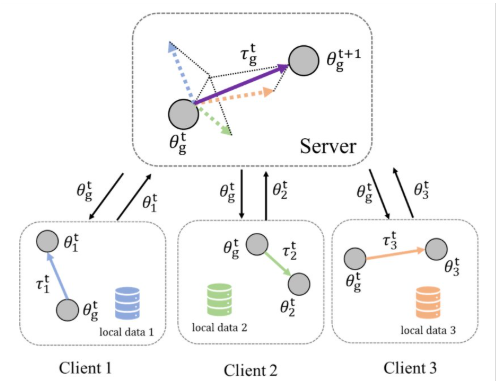
\includegraphics[width=0.8\textwidth]{img/fedawa_mechanism.png}
        \captionof{figure}{Minh họa cơ chế của FedAWA: Các Client Vector (mũi tên nhỏ) có hướng khác nhau do Non-IID. FedAWA tính toán vector tổng hợp tối ưu (mũi tên đậm) sao cho giảm thiểu sự phân kỳ, thay vì chỉ cộng trung bình \cite{Shi2025AWA}.}
        \label{fig:FedAWA}
    \end{minipage}
\end{center}

\subsection{Phân tích Ưu và Nhược điểm}
\begin{itemize}
    \item \textbf{Ưu điểm:}
    \begin{itemize}
        \item \textbf{Khắc phục triệt để Client Drift:} Bằng cách gán trọng số thấp cho các client có vector cập nhật lệch hướng (thường là các client có dữ liệu cực đoan), FedAWA giúp mô hình hội tụ ổn định hơn nhiều so với FedAvg.
        \item \textbf{Công bằng hơn:} Trọng số được quyết định bởi chất lượng đóng góp thay vì số lượng dữ liệu. Điều này đặc biệt hữu ích khi một số client có rất nhiều dữ liệu nhưng chất lượng thấp (rác, nhiễu).
        \item \textbf{Không cần tham số phụ:} Thuật toán hoạt động hoàn toàn dựa trên trọng số mô hình gửi về, không yêu cầu client gửi thêm thống kê loss hay gradient.
    \end{itemize}
    
    \item \textbf{Nhược điểm:}
    \begin{itemize}
        \item \textbf{Chi phí tính toán tại Server cao:} Việc giải bài toán tối ưu hóa tìm $\Lambda^*$ tại mỗi vòng lặp phức tạp hơn nhiều so với phép tính trung bình đơn giản ($O(1)$) của FedAvg. Khi số lượng client $K$ rất lớn, bước này có thể tạo ra nút thắt cổ chai về thời gian xử lý.
    \end{itemize}
\end{itemize}



\section{Thuật toán FedNolowe (Federated Normalized Loss-based Weighted Aggregation)}
\label{sec:FedNolowe}

\subsection{Tổng quan và Động lực nghiên cứu}
\textbf{FedNolowe}, được đề xuất bởi Lê và các cộng sự (2025), đại diện cho một hướng tiếp cận dựa trên hiệu suất (performance-based aggregation) thay vì dựa trên khối lượng dữ liệu \cite{Le2025}.

Động lực của thuật toán xuất phát từ một thực tế trong Học máy liên kết: "Số lượng dữ liệu không đồng nghĩa với chất lượng mô hình". Trong thuật toán FedAvg truyền thống, một client sở hữu lượng dữ liệu lớn nhưng chứa nhiều nhiễu (noisy data) hoặc nhãn sai (incorrect labels) vẫn được gán trọng số cao ($n_k/n$). Điều này khiến mô hình toàn cầu bị "đầu độc" bởi các tri thức sai lệch, dẫn đến quá trình hội tụ không ổn định.

FedNolowe giải quyết vấn đề này bằng giả định: \textit{Giá trị hàm mất mát (Loss value) trên tập dữ liệu cục bộ là thước đo đáng tin cậy nhất cho mức độ "phù hợp" của dữ liệu client đối với tác vụ hiện tại}. Một client có loss thấp nghĩa là mô hình cục bộ đã học tốt, và ngược lại. Do đó, FedNolowe đề xuất cơ chế gán trọng số tỷ lệ nghịch với giá trị loss đã được chuẩn hóa.

\subsection{Cơ chế Chuẩn hóa Loss hai giai đoạn (Two-stage Loss Normalization)}
Quy trình cốt lõi của FedNolowe nằm ở việc chuyển đổi giá trị Loss thô (Raw Loss) từ các client thành trọng số tổng hợp $\alpha_k$. Quá trình này được thực hiện qua 2 giai đoạn toán học chặt chẽ:

{Giai đoạn 1: Chuẩn hóa Quy mô (Scale Normalization)}
Giả sử tại vòng $t$, có tập client tham gia $S_t$. Mỗi client $k$ gửi về máy chủ giá trị loss trung bình cục bộ $\mathcal{L}_k^t$.
Do giá trị loss có thể dao động trong khoảng rất rộng tùy thuộc vào batch size và dữ liệu, máy chủ trước tiên thực hiện chuẩn hóa L1 để đưa loss của tất cả client về cùng một thang đo tỷ lệ (từ 0 đến 1):
\begin{equation}
    \tilde{\mathcal{L}}_k^t = \frac{\mathcal{L}_k^t}{\sum_{j \in S_t} \mathcal{L}_j^t}
\end{equation}
Tại đây, $\tilde{\mathcal{L}}_k^t$ đại diện cho "tỷ trọng sai số" mà client $k$ đóng góp vào tổng sai số của hệ thống.

{Giai đoạn 2: Nghịch đảo và Tái chuẩn hóa (Inversion \& Re-normalization)}
Mục tiêu của chúng ta là: \textbf{Loss càng cao $\to$ Trọng số càng thấp}. Do đó, thuật toán sử dụng phép nghịch đảo dựa trên hiệu số (subtraction-based inversion) để tránh các vấn đề về số học (như chia cho 0).
Giá trị điểm số (score) của client $k$ được tính là phần bù của loss chuẩn hóa: $1 - \tilde{\mathcal{L}}_k^t$.

Cuối cùng, trọng số tổng hợp $\alpha_k^t$ được xác định bằng cách tái chuẩn hóa các điểm số này sao cho tổng trọng số bằng 1:
\begin{equation}
    \alpha_k^t = \frac{1 - \tilde{\mathcal{L}}_k^t}{\sum_{j \in S_t} (1 - \tilde{\mathcal{L}}_j^t)}
\end{equation}
Công thức này đảm bảo rằng các client có loss thấp (hiệu suất tốt) sẽ có $\alpha_k^t$ lớn, đóng góp nhiều hơn vào mô hình toàn cầu. Ngược lại, các client có loss cao bất thường (có thể do dữ liệu nhiễu hoặc tấn công) sẽ bị gán trọng số rất nhỏ, giảm thiểu tác động tiêu cực.

\subsection{Quy trình thực hiện tổng thể}
Tại mỗi vòng giao tiếp $t$:
\begin{enumerate}
    \item \textbf{Huấn luyện và Báo cáo:} Client $k$ thực hiện huấn luyện cục bộ để cập nhật trọng số $w_k^{t+1}$, đồng thời tính toán loss trung bình $\mathcal{L}_k^t$ trên tập dữ liệu của mình. Client gửi cả $w_k^{t+1}$ và $\mathcal{L}_k^t$ về server.
    
    \item \textbf{Tính toán Trọng số:} Server thu thập các giá trị loss, thực hiện quy trình chuẩn hóa 2 giai đoạn như trên để tìm ra bộ trọng số $\{\alpha_k^t\}$.
    
    \item \textbf{Tổng hợp Mô hình:} Server cập nhật mô hình toàn cầu mới:
    \begin{equation}
        w^{t+1} = \sum_{k \in S_t} \alpha_k^t w_k^{t+1}
    \end{equation}
\end{enumerate}
\begin{center}
    \begin{minipage}{\linewidth}
        \centering
        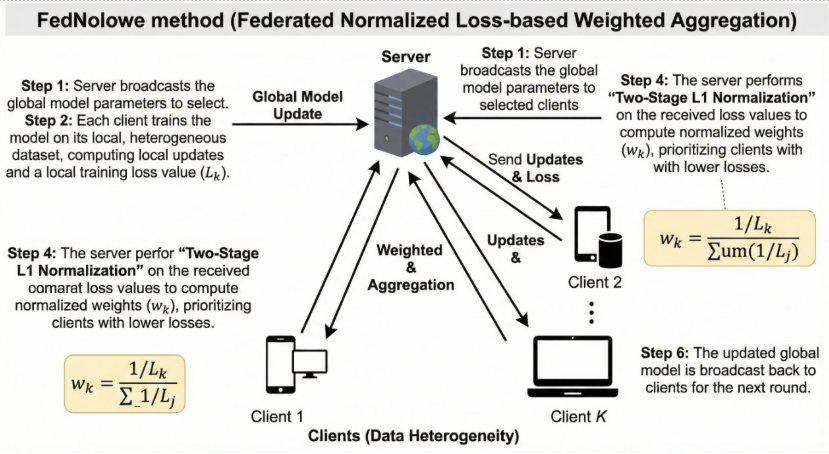
\includegraphics[width=0.85\textwidth]{img/fednolowe_process.png}
        \captionof{figure}{Sơ đồ minh họa quy trình của FedNolowe: Từ Loss cục bộ $\mathcal{L}_k$ được chuyển đổi qua 2 bước chuẩn hóa để tạo ra trọng số $\alpha_k$ tối ưu \cite{Le2025}.}
        \label{fig:fednolowe_process}
    \end{minipage}
\end{center}

\subsection{Phân tích Ưu và Nhược điểm}
\begin{itemize}
    \item \textbf{Ưu điểm:}
    \begin{itemize}
        \item \textbf{Kháng nhiễu tốt (Robustness):} FedNolowe tự động loại bỏ tác động của các client "kém chất lượng" (loss cao), giúp mô hình ổn định hơn trước dữ liệu nhiễu hoặc phân phối Non-IID cực đoan.
        \item \textbf{Hiệu quả tính toán:} Quy trình tính toán trọng số $\alpha_k$ cực kỳ đơn giản (độ phức tạp $O(K)$), nhanh hơn nhiều so với việc giải bài toán tối ưu của FedAWA.
        \item \textbf{Dễ tích hợp:} Có thể áp dụng ngay lập tức vào bất kỳ kiến trúc FL nào mà không cần thay đổi cấu trúc mô hình.
    \end{itemize}
    
    \item \textbf{Nhược điểm:}
    \begin{itemize}
        \item \textbf{Nguy cơ về quyền riêng tư:} Việc gửi giá trị Loss về server có thể rò rỉ một phần thông tin về độ khó của dữ liệu cục bộ (mặc dù ít nghiêm trọng hơn gửi gradient).
        \item \textbf{Phụ thuộc vào tính trung thực:} Nếu một client gian dối báo cáo loss giả mạo (rất thấp) mặc dù không học gì, nó có thể chiếm quyền kiểm soát mô hình toàn cầu (Loss poisoning attack).
    \end{itemize}
\end{itemize}

\section{Thuật toán FedProto (Federated Prototype Learning)}
\label{sec:FedProto}

\subsection{Tổng quan và Động lực nghiên cứu}
\textbf{FedProto (Federated Prototype Learning)}, được giới thiệu bởi Tan và các cộng sự tại hội nghị AAAI 2022, đại diện cho một bước chuyển mình quan trọng trong tư duy thiết kế hệ thống Học máy liên kết \cite{Tan2022}.

Các thuật toán truyền thống như FedAvg, FedLWS hay FedAWA đều dựa trên một giả định cứng nhắc: "Tất cả các client phải sử dụng cùng một kiến trúc mạng nơ-ron (Model Isomorphism)". Tuy nhiên, trong thực tế, các thiết bị tham gia mạng lưới (IoT, điện thoại, máy chủ) có năng lực phần cứng rất khác nhau. Ép buộc một thiết bị IoT yếu ớt chạy cùng mô hình ResNet-50 với một máy chủ mạnh mẽ là điều không khả thi.

FedProto ra đời để giải quyết vấn đề "Tính không đồng nhất về mô hình" (Model Heterogeneity). Thay vì trao đổi tham số mô hình (gradients/weights) - vốn yêu cầu kiến trúc phải giống hệt nhau để thực hiện phép cộng, FedProto đề xuất trao đổi "Tri thức lớp" (Class Prototypes). Điều này cho phép các client sử dụng các mô hình khác nhau (ResNet, CNN, MobileNet...) nhưng vẫn có thể cộng tác học tập thông qua ngôn ngữ chung là các vector đặc trưng lớp.

\subsection{Cơ sở Toán học: Prototype và Cơ chế giao tiếp}

{Định nghĩa Prototype (Mẫu hình)}
Trong FedProto, một \textit{Prototype} của lớp $j$, ký hiệu là $C^{(j)}$, được định nghĩa là vector trung bình của các biểu diễn đặc trưng (embedding vectors) của tất cả dữ liệu thuộc lớp đó.
Giả sử client $k$ có bộ trích xuất đặc trưng (Feature Extractor) $f_k(\cdot)$. Với tập dữ liệu cục bộ $D_{k,j}$ thuộc lớp $j$, prototype cục bộ được tính như sau:
\begin{equation}
    C_k^{(j)} = \frac{1}{|D_{k,j}|} \sum_{(x,y) \in D_{k,j}} f_k(x)
\end{equation}
Prototype này đóng vai trò là "đại diện ngữ nghĩa" cho lớp $j$ tại client $k$.

{Cơ chế Học dựa trên Prototype (Prototype-based Learning)}
Quy trình tối ưu hóa của FedProto không cập nhật trọng số trực tiếp từ server. Thay vào đó, nó sử dụng các Global Prototypes để hướng dẫn quá trình huấn luyện cục bộ thông qua một hàm mất mát điều chuẩn (Regularization Loss).

Hàm mục tiêu cục bộ tại client $k$ được thiết lập như sau:
\begin{equation}
    \min_{\theta_k} \mathcal{L}_{total} = \mathcal{L}_{CE}(\hat{y}, y) + \lambda \cdot \mathcal{L}_{proto}
\end{equation}
Trong đó:
\begin{itemize}
    \item $\mathcal{L}_{CE}$: Hàm mất mát Cross-Entropy tiêu chuẩn để phân loại đúng.
    \item $\mathcal{L}_{proto}$: Hàm mất mát khoảng cách (thường là L2 distance), ép buộc đặc trưng của dữ liệu cục bộ $f_k(x_i)$ phải tiến gần về phía Prototype toàn cầu $\bar{C}^{(y_i)}$ tương ứng với nhãn $y_i$:
    \begin{equation}
        \mathcal{L}_{proto} = \frac{1}{|D_k|} \sum_{(x_i, y_i) \in D_k} \| f_k(x_i) - \bar{C}^{(y_i)} \|_2^2
    \end{equation}
\end{itemize}

\subsection{Quy trình thực hiện thuật toán}
Quy trình của FedProto khác biệt hoàn toàn so với dòng họ FedAvg do không có bước "cộng trọng số".

\begin{enumerate}
    \item \textbf{Huấn luyện và Tính toán Prototype:} Client $k$ huấn luyện mô hình riêng của mình, sau đó tính toán bộ prototype cục bộ $C_k = \{C_k^{(1)}, ..., C_k^{(M)}\}$ cho các lớp dữ liệu mà nó sở hữu.
    
    \item \textbf{Tải lên (Upload):} Client gửi bộ vector $C_k$ về máy chủ.
    \textit{Lưu ý:} Kích thước của vector prototype nhỏ hơn hàng ngàn lần so với bộ tham số mô hình, giúp tiết kiệm băng thông cực lớn.
    
    \item \textbf{Tổng hợp (Aggregation):} Server tổng hợp các prototype cục bộ cùng lớp để tạo ra Prototype toàn cầu:
    \begin{equation}
        \bar{C}^{(j)} = \frac{1}{|S_j|} \sum_{k \in S_j} C_k^{(j)}
    \end{equation}
    với $S_j$ là tập các client có sở hữu dữ liệu lớp $j$.
    
    \item \textbf{Phân phối (Broadcast):} Server gửi bộ Prototype toàn cầu $\bar{C} = \{\bar{C}^{(1)}, ...\}$ về cho các client để sử dụng cho vòng huấn luyện tiếp theo (tính toán $\mathcal{L}_{proto}$).
\end{enumerate}

\begin{center}
    \begin{minipage}{\linewidth}
        \centering
        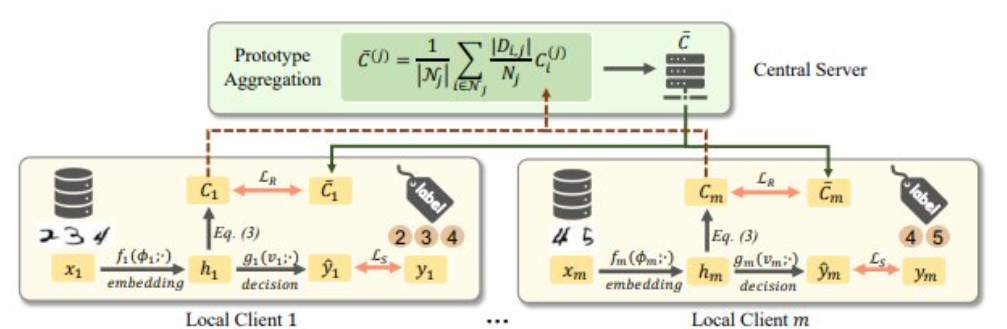
\includegraphics[width=0.9\textwidth]{img/fedproto_framework.png}
        \captionof{figure}{Kiến trúc FedProto: Các client với mô hình khác nhau (Heterogeneous Models) giao tiếp bằng cách gửi các vector Prototype màu sắc về Server thay vì gửi tham số mô hình \cite{Tan2022}.}
        \label{fig:FedProto}
    \end{minipage}
\end{center}
\subsection{Phân tích Ưu và Nhược điểm}
\begin{itemize}
    \item \textbf{Ưu điểm:}
    \begin{itemize}
        \item \textbf{Hỗ trợ Mô hình không đồng nhất:} Đây là ưu điểm độc nhất. Client mạnh có thể dùng ResNet-50, client yếu dùng MobileNetV3, chúng vẫn học được từ nhau.
        \item \textbf{Siêu tiết kiệm băng thông:} Vector prototype (ví dụ: 10 lớp $\times$ 512 chiều) nhỏ hơn rất nhiều so với mô hình (triệu tham số).
        \item \textbf{Bảo mật cao:} Không gửi tham số mô hình đồng nghĩa với việc cực khó để khôi phục lại cấu trúc mạng hay dữ liệu gốc (Gradient Inversion Attack trở nên vô hiệu).
    \end{itemize}
    
    \item \textbf{Nhược điểm:}
    \begin{itemize}
        \item \textbf{Phụ thuộc vào Không gian đặc trưng:} Thuật toán chỉ hoạt động tốt khi các mô hình khác nhau trích xuất ra không gian đặc trưng (embedding space) có cùng số chiều.
        \item \textbf{Hiệu suất trên IID:} Trong trường hợp lý tưởng (IID, mô hình giống nhau), FedProto thường có độ chính xác thấp hơn FedAvg do không tận dụng được việc chia sẻ tham số chi tiết.
        \item \textbf{Vấn đề Missing Class:} Nếu một lớp dữ liệu không xuất hiện ở bất kỳ client nào trong vòng đó, Prototype toàn cầu của lớp đó sẽ không được cập nhật.
    \end{itemize}
\end{itemize}